\chapter{Mathematics}
\noindent
\textbf{A},\textbf{B}, ..., are vector functions\\
$\overleftrightarrow{\textbf{T}}$ is a tensor \\
$\psi$ and $\xi$ are scalar functions\\
$\sigma$ and $\tau$ refer to surfaces and volumes, respectively\\
$d\boldsymbol{\sigma}$ is a differential surface element pointing away from the volume\\
$d\tau$ is a differential volume element\\
$d\boldsymbol{r}$ is a differential line element\\
\index{Vector identities}
\section{Vector Identities}

% The following identities are from the NRL formulary (find  ref.)
\subsection{Identities Involving Only Vectors \scite{huda}{4}}
\renewcommand{\labelenumi}{(\alph{enumi})}
\begin{enumerate}
  \item{$\textbf{A}\cdot\textbf{B}\times\textbf{C} = \textbf{A}\times\textbf{B}\cdot\textbf{C} = \textbf{B}\cdot\textbf{C}\times\textbf{A}$}
  \item{$\textbf{A}\times(\textbf{B}\times\textbf{C}) = (\textbf{C}\times\textbf{B})\times\textbf{A} = \textbf{B}(\textbf{A}\cdot\textbf{C}) - \textbf{C}(\textbf{A}\cdot\textbf{B})$}
  \item{$(\textbf{A}\times\textbf{B})\cdot(\textbf{C}\times\textbf{D}) = (\textbf{A}\cdot\textbf{C})(\textbf{B}\cdot\textbf{D}) - (\textbf{A}\cdot\textbf{D})(\textbf{B}\cdot\textbf{C})$}
  \item{$(\textbf{A}\times\textbf{B})\times(\textbf{C}\times\textbf{D})= \textbf{C}(\textbf{A}\times\textbf{B}\cdot\textbf{D}) - \textbf{D}(\textbf{A}\times\textbf{B}\cdot\textbf{C})$}
\end{enumerate}

% The following identities are taken from Math. Methods in the Phys. Sciece (Boas,1982) p296 and NRL formulary
\subsection{Identities Involving $\nabla$ \scite{huda}{4} \textnormal{\cite{griffiths}}}
\renewcommand{\labelenumi}{(\alph{enumi})}
\begin{enumerate}
  \item{$\nabla \cdot (\psi\textbf{A}) = \psi(\nabla\cdot\textbf{A}) + \textbf{A} \cdot (\nabla\psi)$}
  \item{$\nabla \times (\psi\textbf{A}) = \psi(\nabla \times \textbf{A}) - \textbf{A}\times(\nabla\psi)$}
  \item{$\nabla \cdot (\textbf{A} \times \textbf{B}) = \textbf{B} \cdot (\nabla \times \textbf{A}) - \textbf{A} \cdot (\nabla \times \textbf{B})$}
  \item{$\nabla \times (\textbf{A} \times \textbf{B}) = (\textbf{B} \cdot \nabla)\textbf{A} - (\textbf{A} \cdot \nabla)\textbf{B} + \textbf{A}(\nabla \cdot \textbf{B}) - \textbf{B}(\nabla \cdot \textbf{A})$}
  \item{$\nabla(\textbf{A}\cdot\textbf{B}) = \textbf{A} \times (\nabla \times \textbf{B}) + \textbf{B}\times(\nabla\times\textbf{A}) + (\textbf{A}\cdot\nabla)\textbf{B} + (\textbf{B}\cdot\nabla)\textbf{A}$}
  \item{$\nabla\cdot(\textbf{A}\textbf{B}) = (\nabla \cdot \textbf{A})\textbf{B} +(\textbf{A}\cdot\nabla)\textbf{B}$}
  \item{$\nabla \cdot (\psi\overleftrightarrow{\textbf{T}}) = \nabla\psi\cdot\overleftrightarrow{\textbf{T}} + \psi\nabla\cdot\overleftrightarrow{\textbf{T}}$}
  \item{$\nabla \cdot (\nabla \times \textbf{A}) = 0$}
  \item{$\nabla^2\textbf{A} = \nabla(\nabla\cdot\textbf{A}) - \nabla\times\nabla\times\textbf{A}$}
  \item{$\nabla(\psi\xi) = \nabla(\phi\xi) = \psi\nabla\xi + \xi\nabla\psi$}
  \item{$\nabla\cdot(\nabla\psi\times\nabla\xi) = 0$}
  \item{$\nabla \cdot \nabla\psi = \nabla^2\psi$}
  \item{$\nabla \times \nabla\psi = 0$}

\end{enumerate}

% The following identities are taken from Math. Methods in the Phys. Sciece (Boas,1982) p293
\subsection{Identities Involving $\int$ \scite{huda}{5}}
\fla{ \text{(a)}& \int\limits_{volume}\!\!\! \nabla\psi\,d\tau =\!\!\! \int\limits_{surface}\!\!\!\! \psi\,d\boldsymbol{\sigma} &}

\fla{ \text{(b)}& \int\limits_{volume}\!\!\!\! \nabla\times\textbf{A}\,d\tau =\!\!\! \oint\limits_{surface}\!\!\!\!\! d\boldsymbol{\sigma}\times\textbf{A}&}

\fla{ \text{(c)}& \int\limits_{surface}\!\!\!\!\! d\boldsymbol{\sigma}\cdot\nabla\times\textbf{A} =\!\!\! \oint\limits_{boundary}\!\!\!\!\! d\boldsymbol{r}\cdot\textbf{A} & }

\fla{ \text{(d)}& \oint\limits_{boundary}\!\!\!\!\! d\textbf{r}\times\textbf{A} =\!\!\! \int\limits_{surface}(d\boldsymbol{\sigma}\times\nabla)\times\textbf{A} & }


\section{Curvilinear Coordinate Systems}

% Needs verification and sound mathematical reference
\index{Cylindrical coordinate systems}
\subsection{Cylindrical Coordinates $\left(r,\theta,z\right)$ \scite{huda}{6-7} \textnormal{\cite{griffiths}}}

\noindent
Differential volume: $d\tau = r\,dr\,d\theta\,dz$
\\[3pt]

\noindent
Relation to cartesian coordinates:
\flatwo{
  x &= r\cos\theta & \boldsymbol{\hat{x}} &= \cos\phi\,\boldsymbol{\hat{r}} - \sin\phi\,\boldsymbol{\hat{\phi}} &\\
  y &= r\sin\theta & \boldsymbol{\hat{y}} &= \sin\phi\,\boldsymbol{\hat{r}} + \cos\phi\,\boldsymbol{\hat{\phi}} &\\
  z &= z           & \boldsymbol{\hat{z}} &= \boldsymbol{\hat{z}} &
}{4}


\noindent
Unit vector differentials
\flatwo{
  \frac{d\boldsymbol{\hat{r}}}{dt} &= \boldsymbol{\hat{\theta}}\frac{d\theta}{dt} &
  \frac{d\boldsymbol{\hat{\theta}}}{dt} &= -\boldsymbol{\hat{r}}\frac{d\theta}{dt}
}{7}

\noindent
Gradient
\fla{ \nabla \psi &= \frac{\partial \psi}{\partial r} \boldsymbol{\hat{r}} + \frac{1}{r} \frac{\partial \psi}{\partial \theta} \boldsymbol{\hat{\theta}} + \frac{\partial \psi}{\partial z} \boldsymbol{\hat{z}} &}


\noindent
Divergence 
\fla{ \nabla \cdot \textbf{A} &= \frac{1}{r}\frac{\partial}{\partial r}\left(rA_r\right) + \frac{1}{r}\frac{\partial A_\theta}{\partial\theta} + \frac{\partial A_z}{\partial z} &}

\noindent
Curl
\fla{
  \nabla \times \textbf{A} &= \left(\frac{1}{r}\frac{\partial A_z}{\partial \theta} - \frac{\partial A_\theta}{\partial z}\right)\boldsymbol{\hat{r}} \\
  &+ \left(\frac{\partial A_r}{\partial z} - \frac{\partial A_z}{\partial r}\right)\boldsymbol{\hat{\theta}} \\
  &+ \left(\frac{1}{r} \frac{\partial}{\partial r}\left(rA_\theta\right) - \frac{1}{r} \frac{\partial A_r}{\partial \theta}\right)\boldsymbol{\hat{z}} &
}

\noindent
Laplacian
\fla{
  \nabla^2 \psi &= \frac{1}{r}\frac{\partial}{\partial r}\left(r\frac{\partial \psi}{\partial r}\right) + \frac{1}{r^2}\frac{\partial^2 \psi}{\partial \theta^2}
+ \frac{\partial^2 \psi}{\partial z^2} &}

\noindent
Vector-dot-grad 
\fla{
  \left(\textbf{A} \cdot \nabla \right)\textbf{B} &= \left(A_r \frac{\partial B_r}{\partial r} + \frac{A_\theta}{r} \frac{\partial B_r}{\partial\theta}
  + A_z \frac{\partial B_r}{\partial z} - \frac{A_\theta B_\theta}{r}\right)\boldsymbol{\hat{r}} \\
  &+ \left(A_r\frac{\partial B_\theta}{\partial r} + \frac{A_\theta}{r}\frac{\partial B_\theta}{\partial \theta} + A_z\frac{\partial B_\theta}{\partial z} + \frac{A_\theta B_r}{r}\right)\boldsymbol{\hat{\theta}} \\
  &+ \left(A_r\frac{\partial B_z}{\partial r} + \frac{A_\theta}{r}\frac{\partial B_z}{\partial \theta} + A_z\frac{\partial B_z}{\partial z}\right)\boldsymbol{\hat{z}} &
}

% Needs verification and sound mathematical reference
\index{Spherical coordinate systems}
\subsection{Spherical Coordinates $\left(r,\theta,\phi\right)$ \scite{huda}{8-9} \textnormal{\cite{griffiths}}}

Differential volume: $d\tau = r^2\,\sin\theta\,dr\,d\theta\,d\phi$
\\[3pt]

\noindent
Relation to cartesian coordinates
\flatwo{
  x &= r\sin\theta\cos\phi & \boldsymbol{\hat{x}} &= \sin\theta\cos\phi\,\boldsymbol{\hat{r}} + \cos\theta\cos\phi\,\boldsymbol{\hat{\theta}} - \sin\phi\,\boldsymbol{\hat{\phi}} &\\
  y &= r\sin\theta\sin\phi & \boldsymbol{\hat{y}} &= \sin\theta\sin\phi\,\boldsymbol{\hat{r}} + \cos\theta\sin\phi\,\boldsymbol{\hat{\theta}} + \cos\phi\,\boldsymbol{\hat{\phi}} &\\
  z &= r\cos\theta         & \boldsymbol{\hat{z}} &= \cos\theta\,\boldsymbol{\hat{r}} - \sin\theta\,\boldsymbol{\hat{\theta}} &\\
}{1}

\noindent
Gradient
\fla{ \nabla \psi &= \frac{\partial \psi}{\partial r} \boldsymbol{\hat{r}} + \frac{1}{r}\frac{\partial \psi}{\partial\theta} \boldsymbol{\hat{\theta}} + \frac{1}{r\sin\theta}\frac{\partial \psi}{\partial \phi} \boldsymbol{\hat{\phi}} &}

\noindent
Divergence
\fla{ \nabla \cdot \textbf{A} &= \frac{1}{r^2}\frac{\partial}{\partial r}\left(r^2A_r\right) + \frac{1}{r\sin\theta}\frac{\partial}{\partial\theta}\left(\sin\theta A_\theta\right) + \frac{1}{r\sin\theta}\frac{\partial A_\phi}{\partial \phi} &}

\noindent
Curl
\fla{
  \nabla \times \textbf{A} &= \left(\frac{1}{r\sin\theta}\frac{\partial}{\partial \theta}\left(\sin\theta A_\phi\right) - \frac{1}{r\sin\theta}\frac{\partial A_\theta}{\partial \phi}\right)\boldsymbol{\hat{r}} \\
  &+ \left(\frac{1}{r\sin\theta}\frac{\partial A_r}{\partial \phi} - \frac{1}{r}\frac{\partial}{\partial r}\left(rA_\phi\right)\right)\boldsymbol{\hat{\theta}} \\
  &+ \left(\frac{1}{r}\frac{\partial}{\partial r}\left(rA_\theta\right) - \frac{1}{r}\frac{\partial A_r}{\partial \theta}\right)\boldsymbol{\hat{\phi}} &
}

\noindent
Laplacian
\fla{ \nabla^2\psi &= \frac{1}{r^2}\frac{\partial}{\partial r}\left(r^2\frac{\partial \psi}{\partial r}\right) + \frac{1}{r^2\sin\theta}\frac{\partial}{\partial\theta}\left(\sin\theta\frac{\partial\psi}{d\theta}\right) + \frac{1}{r^2\sin^2\theta}\frac{\partial^2\psi}{\partial\phi^2} &}


\noindent
Vector-dot-grad
\fla{
  \left(\textbf{A}\cdot\nabla\right)\textbf{B} &= \left(A_r\frac{\partial B_r}{\partial r} + \frac{A_\theta}{r}\frac{\partial B_r}{\partial\theta} + \frac{A_\phi}{r\sin\theta}\frac{\partial B_r}{\partial\phi} - \frac{A_\theta B_\theta + A_\phi B_\phi}{r}\right)\boldsymbol{\hat{r}} \\
  &+\left(A_r\frac{\partial B_\theta}{\partial r} + \frac{A_\theta}{r}\frac{\partial B_\theta}{\partial\theta} + \frac{A_\phi}{r\sin\theta}\frac{\partial B_\theta}{\partial\phi} + \frac{A_\theta B_r}{r} - \frac{\cot\theta A_\phi B_\phi}{r}\right)\boldsymbol{\hat{\theta}} \\
  &+\left(A_r\frac{\partial B_\phi}{\partial r} + \frac{A_\theta}{r}\frac{\partial B_\phi}{\partial \theta} + \frac{A_\phi}{r\sin\theta}\frac{\partial B_\phi}{\partial\phi} + \frac{A_\phi B_r}{r} + \frac{\cot\theta A_\phi B_\theta}{r}\right)\boldsymbol{\hat{\phi}} &
}

\section{Integral Relations of Vector Calculus}
In this section, let \textbf{A} $\equiv$ \textbf{A}(x$_i$,x$_j$,x$_k$) be a vector function that defines a vector field. \\

\index{Fundamental theorem of calculus}
\subsection{The Fundamental Theorem of Calculus}
If $f(x)$ is a single-valued function on the interval [a,b] \scite{jeffrey}{88}
\fla{ \int_a^bf(x)d x &= F(b) - F(a) &}

\index{Gauss's theorem}
\index{Divergence theorem|see{Gauss's theorem}}
\subsection{Gauss's (or the Divergence) Theorem}
If $\tau$ is a volume enclosed by a surface $\sigma$, where $\boldsymbol{d \sigma} = \boldsymbol{\hat{n}} d\sigma$ and $\boldsymbol{\hat{n}}$ is a unit vector pointing away from $\tau$ \scite{griffiths}{31}
\fla{ \int \limits_{volume}\!\!\!\!\! \left(\nabla \cdot \textbf{A}\right) \, d \tau \, &= \!\!\!\! \oint\limits_{surface}\!\!\!\!\! \textbf{A} \cdot \textbf{d$\boldsymbol\sigma$} &}

\index{Stoke's theorem}
\index{Curl theorem|see{Stoke's theorem}}
\subsection{Stoke's (or the Curl) Theorem}
If $\sigma$ is an open surface defined by a boundary contour at the surface edge \scite{griffiths}{34}
\fla{ \int\limits_{surface}\!\!\!\!\! \left(\nabla \times \textbf{A}\right) \cdot \textbf{d$\boldsymbol\sigma$} \, &= \!\!\!\!\!\! \oint\limits_{contour}\!\!\!\!\!\! \textbf{A} \cdot d\textbf{r} &}


\index{Legendre polynomials}
\section{Legendre Polynomials}

\index{Equations! Legendre's equation}
\index{Legendre's equation}
\noindent
Legendre's equation \scite{jeffrey}{337}
\fla{ &(1-x^2)\frac{d^2y}{dx^2} - 2x\frac{dy}{dx} + l(l+1)y = 0 \hspace{1cm} -1\le x \le 1 \text{  and  } l=0,1,2,\cdots &}

\noindent
\begin{table}[h!]
  \begin{tabular}{c l}
    \multicolumn{2}{c}{Legendre Polynomials \scite{jeffrey}{289}}\\
    \hline
    Order \T\B& Corresponding polynomial\\
    \hline\hline
    $l=0$ \T& $P_0(x) = 1$ \\[3pt]
    $l=1$ & $P_1(x) = x$ \\[3pt]
    $l=2$ & $P_2(x) = \frac{1}{2}(3x^2 - 1)$ \\[3pt]
    $l=3$ & $P_3(x) = \frac{1}{2}(5x^3 - 3x)$ \\[3pt]
    $l=4$ & $P_4(x) = \frac{1}{8}(35x^4 - 30x^2 + 3)$ \\[3pt]
    $l=5$ & $P_5(x) = \frac{1}{8}(63x^5 - 70x^3 + 15x)$ \\[3pt]
    $\cdots$ \B& $\cdots$\\
    \hline
  \end{tabular}
\end{table}

\index{Rodrigues' formula}
\noindent
Rodrigues' formula \scite{jeffrey}{286}
\fla{ P_l(x) &= \frac{1}{2^ll!}\frac{d^l}{dx^l}(x^2-1)^l &}

\noindent
Orthonormality \scite{jeffrey}{286}
\fla{ \int_{-1}^1 P_l(x)P_m(x)\,dx &= \int_0^\pi P_l(\cos\theta)P_m(\cos\theta)\sin\theta\,d\theta 
  = \frac{2}{2l+1}\delta_{lm} &}
\indent where $\delta_{lm}$ is the Kronecker delta: $l=m, \delta_{lm}=1; l\not=m, \delta_{lm}=0$.


% Most of following information came from Jeffrey, A. Chapter 17.

\section{Bessel Functions}

\index{Bessel functions! equation}
\index{Equations! Bessel's equation}
\subsection{Bessel's Equation}
\noindent
The most general form of Bessel's equation is \scite{jeffrey}{269}

\fla {&\frac{d^2y}{dx^2} + \frac{1}{x}\frac{dy}{dx} + \left(\lambda^2 - \frac{p^2}{x^2}\right)y = 0 &}
\noindent
which has the general solution \scite{jeffrey}{270} \fla{y &= AJ_p(\lambda x) +
BY_p(\lambda x) &} where $J_p$ are Bessel functions of the first kind
and $Y_p$ are Bessel functions of the second kind (also known as
Neumann Functions $N_p$), both of order $p$.  Bessel functions of the
first kind have no closed form representation; however, they can be
used to define Bessel functions of the second kind: \scite{jeffrey}{270}

\fla{Y_p(x) &= \frac{J_p(x)\cos(p\pi) - J_{-p}(x)}{\sin(p\pi)} &}

\index{Bessel functions! Useful relations}
\subsection{Bessel Function Relations}
The following relationships are also valid for $Y_p(x)$ by replacing
$J_p(x)$ with $Y_p(x)$ \scite{jeffrey}{278-279}

\fla{
  &\text{(a)  }J_2(x) = \frac{2}{x}J_1(x) - J_0(x) &\\
  &\text{(b)  }\frac{d}{dx}[J_0(x)] = -J_1(x) &\\
  &\text{(c)  }\frac{d}{dx}[x^pJ_p(x)] = x^pJ_{p-1}(x) &\\
  &\text{(d)  }\frac{d}{dx}[x^{-p}J_p(x)] = -x^{-p}J_{p+1}(x) &\\
  &\text{(e)  }J_{p-1}(x) + J_{p+1}(x) = \frac{2p}{x}J_p(x) &\\
  &\text{(f)  }J_{p-1}(x) - J_{p+1}(x) = 2\frac{d}{dx}J_p(x) &\\
  &\text{(g)  }\frac{d}{dx}J_p(x) = -\frac{p}{x}J_p(x) + J_{p-1}(x) = \frac{p}{x}J_p(x) - J_{p+1}(x) &
}

% References: Abromowitz & Stegun, Jaffries
\index{Bessel functions! Asymptotic forms}
\subsection{Asymptotic forms of Bessel Functions}
For $x\rightarrow \infty$\scite{jeffrey}{273}
\fla{
  J_p(x) &\approx \sqrt{\frac{2}{\pi x}}\left[\cos\left(x - \frac{1}{2}p\pi - \frac{1}{4}\pi\right)\right] &\\[6pt]
  Y_p(x) &\approx \sqrt{\frac{2}{\pi x}}\left[\sin\left(x - \frac{1}{2}p\pi - \frac{1}{4}\pi\right)\right] & 
}

\noindent
For $p\rightarrow \infty$ \scite{jeffrey}{273}
\flatwo{
  J_p(x) &\approx \frac{1}{\sqrt{2\pi p}}\left(\frac{ex}{2p}\right)^p &
  Y_p(x) \approx -\sqrt{\frac{2}{\pi p}}\left(\frac{ex}{2p}\right)^{-p} 
}{3}

\index{Bessel functions! Plots}
\begin{figure}[h!]
  \centering
  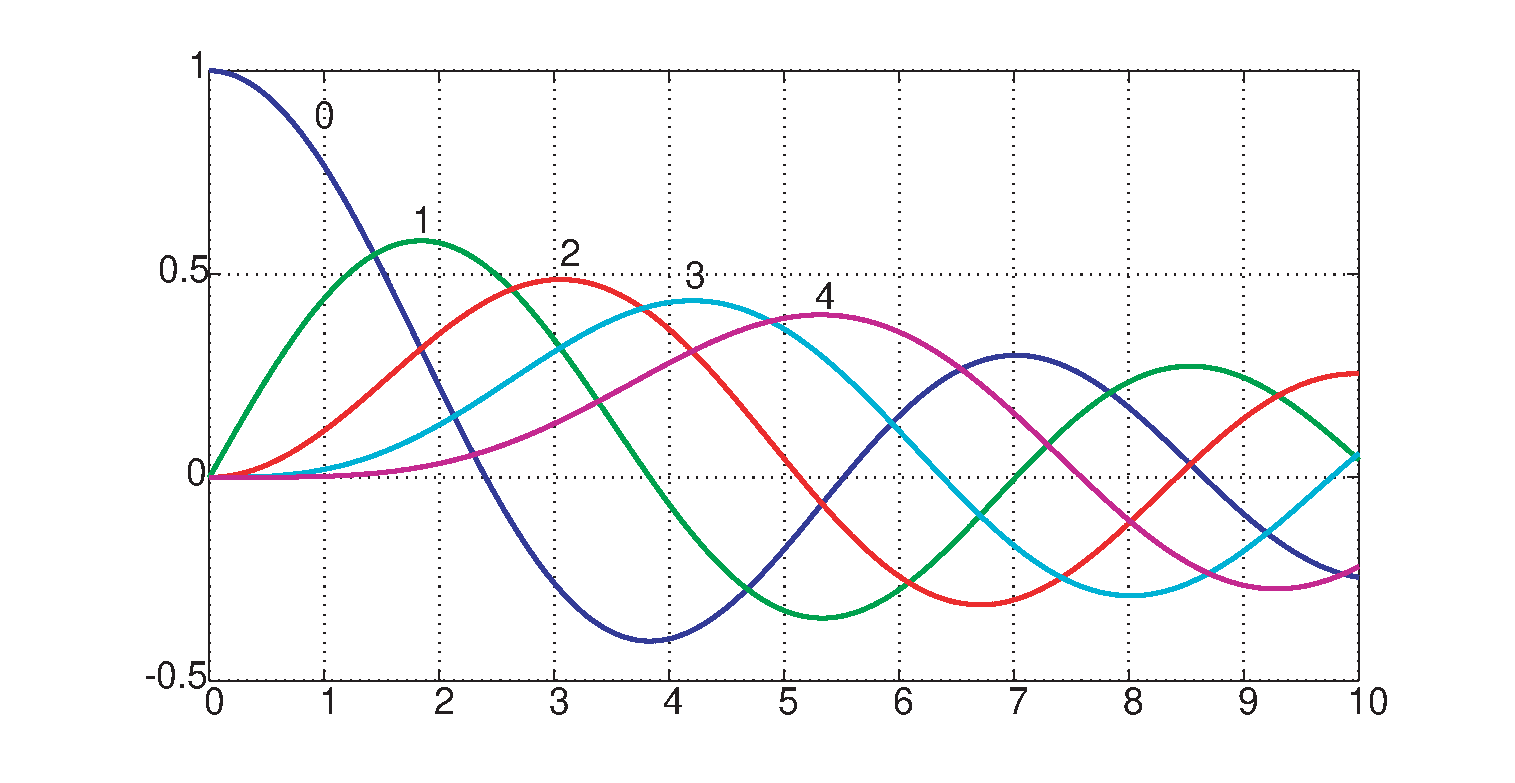
\includegraphics[scale=.45]{figures/besselfirstkind.eps}
  \caption*{\small Plots of $J_{p}(x)$}
\end{figure}

\begin{figure}[h!]
  \centering
  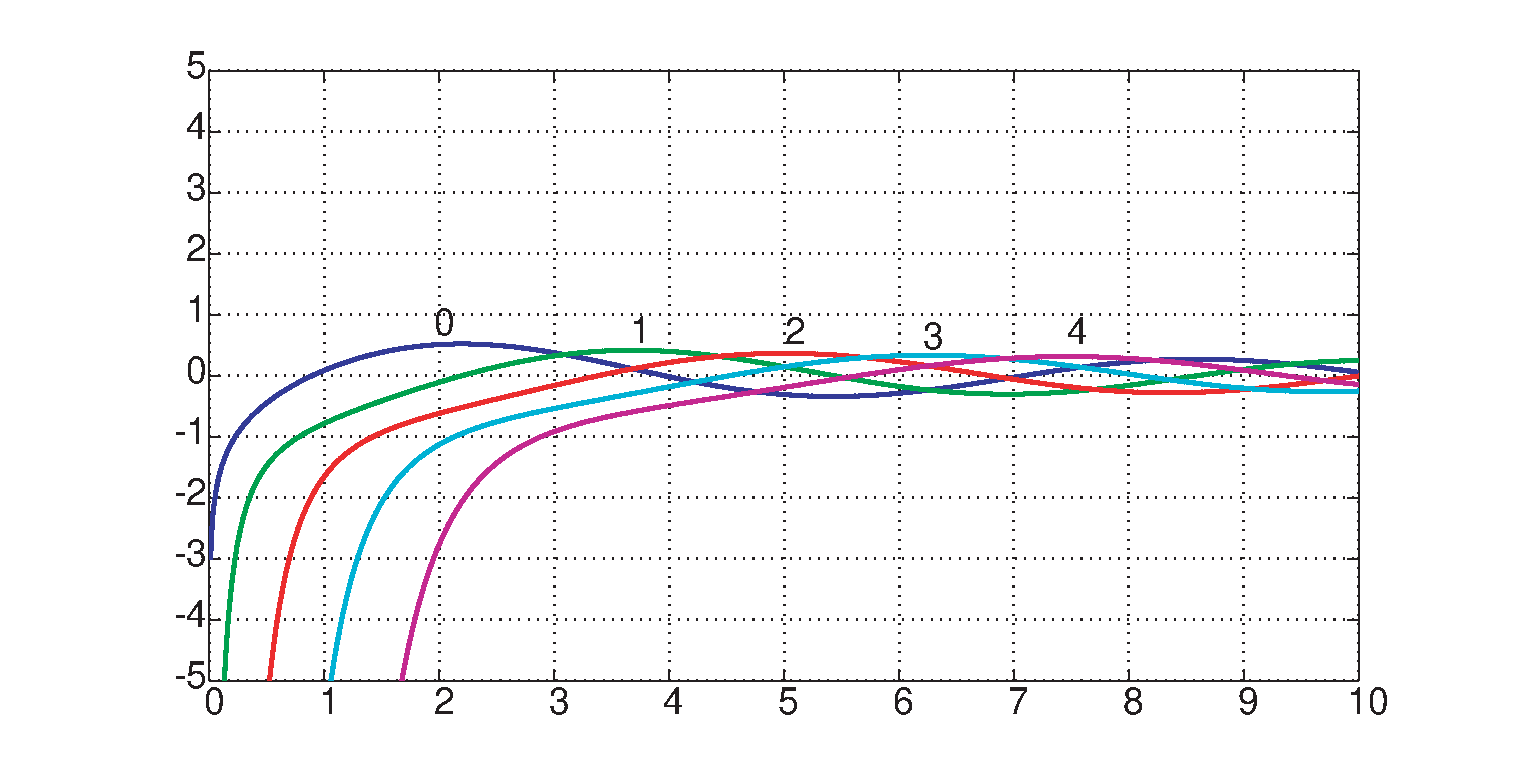
\includegraphics[scale=.45]{figures/besselsecondkind.eps}
  \caption*{\small Plots of $Y_{p}(x)$}
\end{figure}

\section{Modified Bessel Functions}

\index{Bessel functions! Modified equation}
\subsection{Bessel's Modified Equation}
The most general form of Bessel's modified equation is\scite{jeffrey}{274}
\begin{flalign*}
  \indent
  &\frac{d^2y}{dx^2} + \frac{1}{x}\frac{dy}{dx} - \left(\lambda^2 + \frac{p^2}{x^2}\right)y = 0 &
\end{flalign*}
\indent
which has the general solution \scite{jeffrey}{275}
\begin{flalign*}
  \indent
  y &= AI_p(\lambda x) + BK_p(\lambda x) & 
\end{flalign*}
\noindent
where $I_p$ are Modified Bessel functions of the first kind and $K_p$ are modified 
Bessel functions of the second kind.  Modified Bessel functions of the first kind have no
closed form representation; however, they can be used to define Bessel functions of the second kind: \scite{jeffrey}{275}

\fla{K_p(x) &= \frac{\pi}{2} \frac{I_{-p}(x) - I_{p}(x)}{\sin(p\pi)} &}

\index{Bessel functions! Modified useful relations}
\subsection{Modified Bessel Functions Relations}
Relations involving $I_p(x)$ \scite{jeffrey}{280}
\begin{flalign*}
  \indent
  &\text{(a)   }xI_{p-1}(x) - xI_{p+1}(x) = 2pI_p(x) &\\
  &\text{(b)   }I_{p-1}(x) - I_{p+1}(x) = 2 \frac{d}{dx}I_p(x) &\\
  &\text{(c)   }x\frac{d}{dx}\left[I_p(x)\right] + pI_p(x) = xI_{p-1}(x) &\\
  &\text{(d)   }x\frac{d}{dx}\left[I_p(x)\right] - pI_p(x) = xI_{p+1}(x) &\\
  &\text{(e)   }\frac{d}{dx}\left[I_0(x)\right] = I_1(x) &\\
  &\text{(f)   }I_2(x) = - \frac{2}{x}I_1(x) + I_0(x) &\\
\end{flalign*}

\noindent
Relations involving $K_p(x)$ \scite{jeffrey}{280}
\begin{flalign*}
  \indent
  &\text{(g)   }xK_{p-1}(x) - xK_{p+1}(x) = -2pK_p(x) &\\
  &\text{(h)   }K_{p-1}(x) + K_{p+1}(x) = -2 \frac{d}{dx}K_p(x) &\\
  &\text{(i)   }x\frac{d}{dx}\left[K_p(x)\right] + pK_p(x) = -xK_{p-1}(x) &\\
  &\text{(j)   }x\frac{d}{dx}\left[K_p(x)\right] - pK_p(x) = -xK_{p+1}(x) &\\
  &\text{(k)   }\frac{d}{dx}\left[K_0(x)\right] = -K_1(x) &\\
  &\text{(l)   }K_2(x) = \frac{2}{x}K_1(x) + K_0(x) &\\
\end{flalign*}

\index{Bessel functions! Modified asymptotic forms}
\subsection{Asymptotic Forms of Modified Bessel Functions}
For $x\rightarrow\infty$ \scite{jeffrey}{278}
\begin{flalign*}
  \indent
  I_p(x) &\approx \frac{e^x}{\sqrt{2\pi x}}\left(1 - \frac{4p^2-1}{8x}\right) &\\
  K_p(x) &\approx \sqrt{\frac{\pi}{2x}}e^{-x}\left(1 + \frac{4p^2 - 1}{8x}\right) &
\end{flalign*}

\begin{figure}[h!!]
  \centering
  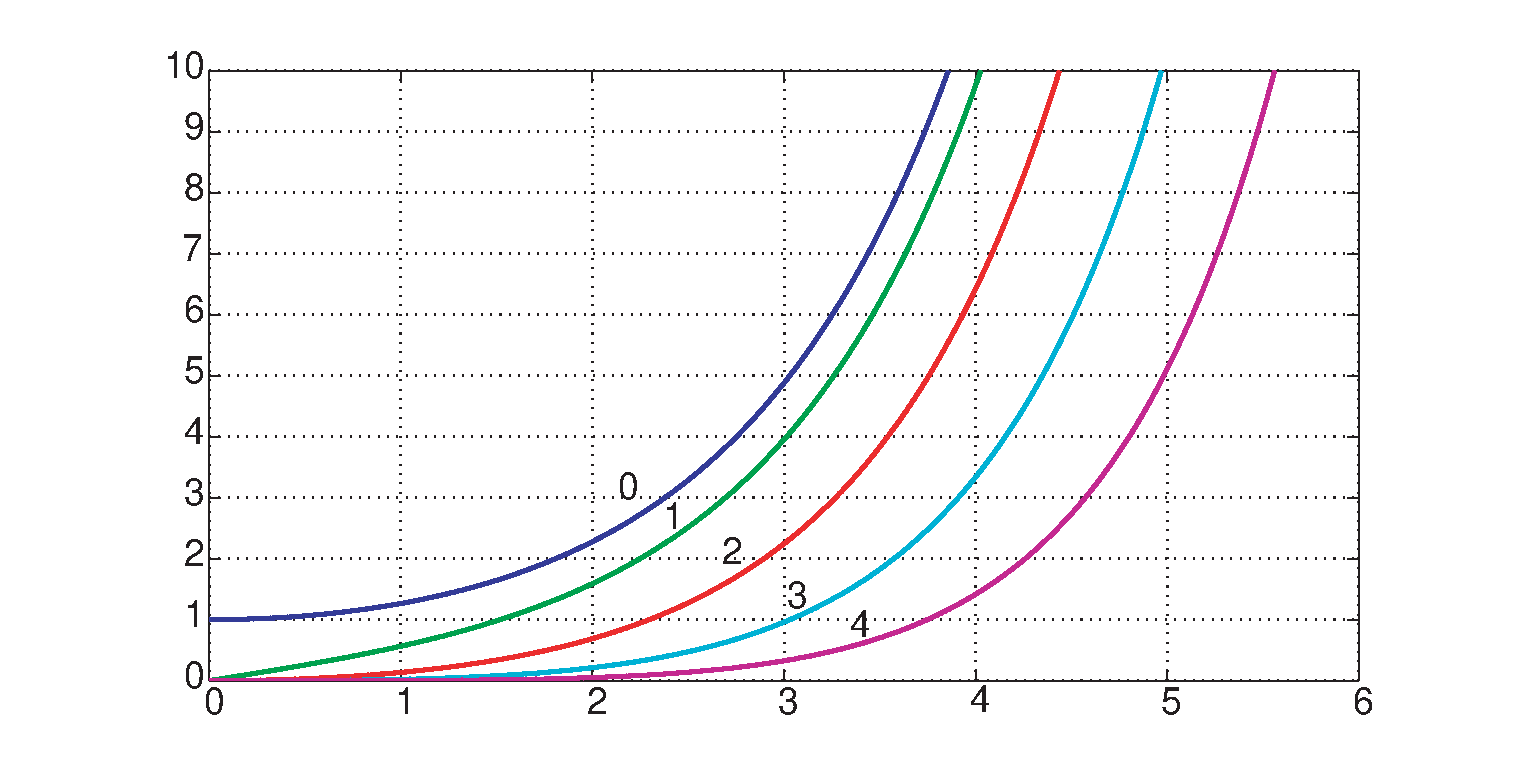
\includegraphics[scale=.45]{figures/modifiedbesselfirstkind.eps}
  \caption*{\small Plots of $I_{p}(x)$ }
\end{figure}

\begin{figure}[h!!]
  \centering
  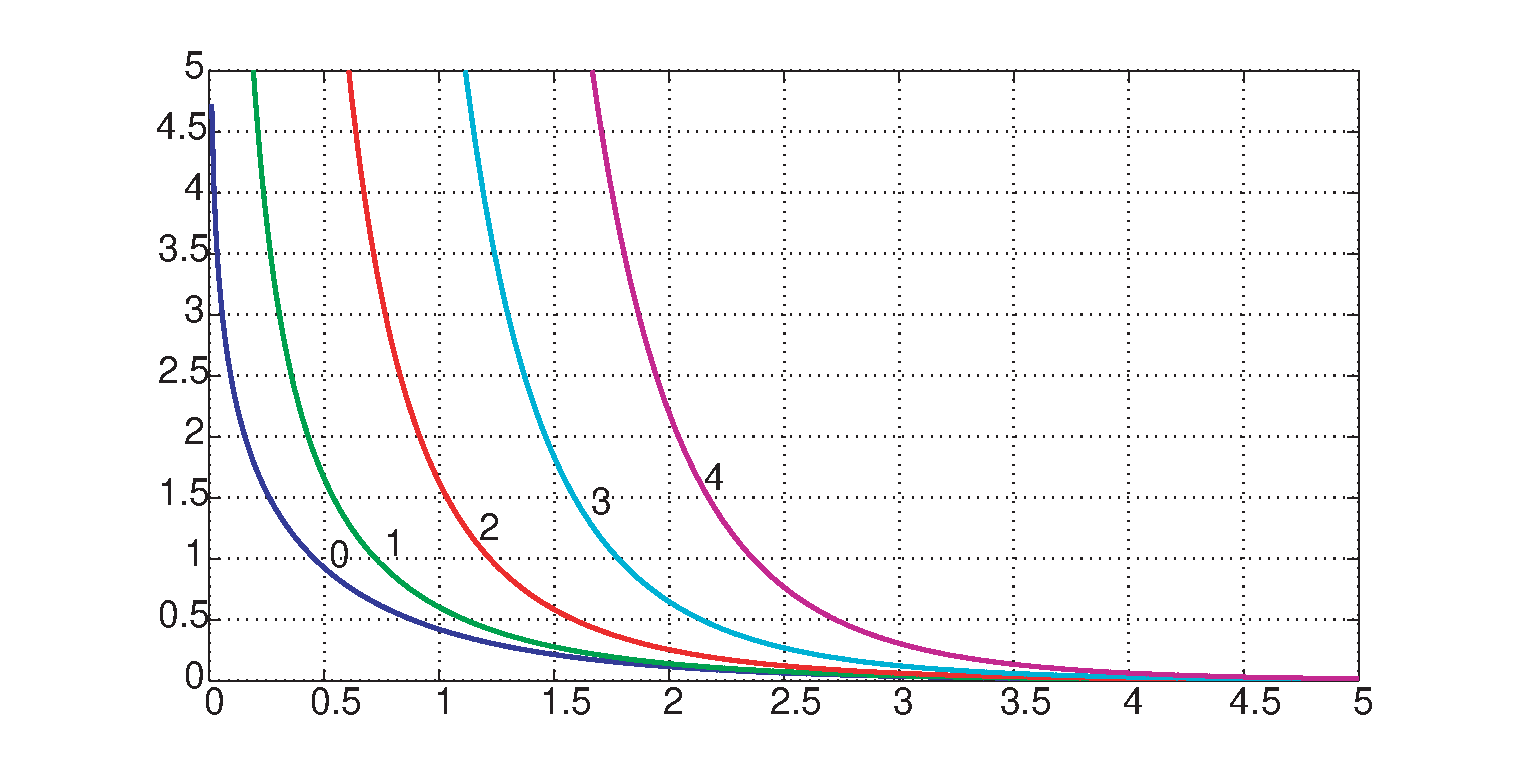
\includegraphics[scale=.45]{figures/modifiedbesselsecondkind.eps}
  \caption*{\small Plots of $K_{p}(x)$}
\end{figure}

\index{Partial differential equations}
\section{Partial Differential Equations}

\index{Basis functions of Laplace's equation}
\subsection{Basis Functions for Laplace's Equation}
%Section from R. Parker notes, 09/11.2008 22.101 MIT Class
Basis functions are the most general solutions to $\nabla^2\psi=0$. \cite{parker}

\renewcommand{\thefootnote}{\fnsymbol{footnote}}

\begin{table}[h!]
  \centering
  \begin{tabular}{ l l}
    \hline
    Geometry \T\B& Basis Function $\psi$\\ 
    \hline\hline
    2D Cartesian \T& $\psi = \left( A \sin kx + B \cos kx \right) \left( C e^{ky} + D e^{-ky} \right) $ \\[5pt]
    2D Cylindrical & $\psi = A_{0} + B_{0} \ln r + \left( A \sin n \theta + B \cos n \theta \right) \times \left( C r^{n} + D r^{-n} \right)$ \\[5pt]
    3D Cartesian   & $\psi = A e^ {ik_{x} x} e^{i k_{y} y} e^{k_{z} z} $ with $k_{x}^{2} + k_{y}^{2} - k_{z}^{2} = 0$ \\[5pt]
    3D Cylindrical & $\psi = A e^{ \pm i m \theta} e^{\pm k z} J_{\pm m}(kr)$ \footnotemark[1] \\[5pt]
    2D Spherical   & $\psi = \left( A r^{l} + B r^{-(l+1)} \right) P_{l}(\cos \theta)$\\[5pt]
    3D Spherical \B& $\psi = \sum\limits_{m=-l}^{l} \left( A_{lm} r^{l} + B_{lm} r^{-(l+1)} \right) Y_{lm}(\theta, \phi)$\footnotemark[2] \\[5pt]
    \hline
\end{tabular}
\end{table}

\footnotetext[1]{\scriptsize If m is an integer, $J_{-m} \rightarrow Y_{m}$. If k is imaginary, $J_{m}(kr) \rightarrow I_{m}(\left| k
      \right| r)$ and $Y_{m}(kr) \rightarrow K_{m}(\left|k \right| r)$}

\footnotetext[2]{\scriptsize $Y_{lm}(\theta, \phi)$ is the spherical
harmonic function}

\renewcommand{\thefootnote}{\arabic{footnote}}

\index{Gaussian integrals}
\section{Gaussian Integrals } %jeffrey 255, placing it in the section causes an error

Definite integral relations of Gaussian integrals \scite{jeffrey}{255}
\fla{
  \indent
  \text{(a)   }&\int_0^\infty e^{-ax^2}dx = \frac{1}{2}\left(\frac{\pi}{a}\right)^{1/2} &\\
  \text{(b)   }&\int_{-\infty}^\infty e^{-ax^2}dx = \left(\frac{\pi}{a}\right)^{1/2} &\\
  \text{(c)   }&\int_{-\infty}^\infty e^{-ax^2}e^{-2bx}dx = \left(\frac{\pi}{a}\right)^{1/2}e^{\frac{b^2}{a}} \hspace{0.5cm}\text{for a$>$0}\\
  \text{(d)   }&\int_{-\infty}^\infty xe^{-a(x-b)x^2}dx = b\left(\frac{\pi}{a}\right)^{1/2} &\\
  \text{(e)   }&\int_{-\infty}^\infty x^2e^{-ax^2}dx = \frac{1}{2}\left(\frac{\pi}{a^3}\right)^{1/2} &\\
  \text{(f)   }&\int_0^\infty x^ne^{-ax^2}dx = \left\{
  \begin{gathered} 
    \frac{1}{2}\Gamma \left(\frac{n+1}{2}\right)/a^{(n+1)/2} \hspace{1cm}\hfill \text{a$>$0} \\
    \frac{(2k-1)!!}{2^{k+1}a^k}\sqrt{\frac{\pi}{a}} \hfill \text{n=2k,a$>$0} \\
    \frac{k!}{2a^{k+1}} \hfill \text{n=2k+1,a$>$0} \\
  \end{gathered} \right.
  &
}

\begin{table}[!h]
  \centering
  \begin{tabular}{c c c c}
    \multicolumn{4}{c}{Definite integrals of common Gaussian relations \scite{stangeby}{65}}\\
    \hline
    n \T\B& $\int \limits_{0}^{\infty} x^ne^{-ax^2}\,dx$ & $\int \limits_{-\infty}^{\infty}x^ne^{-ax^2}\,dx$ & $\int \limits_{0}^{\infty} x^{\frac{1}{2}\left(n-1\right)}e^{-ax}\,dx$\\[6pt]
    \hline\hline
    0 \T& $\frac{\pi^{1/2}}{2a^{1/2}}    $& $\frac{\pi^{1/2}}{a^{1/2}}    $& $\frac{\pi^{1/2}}{a^{1/2}}    $ \\[6pt]
    1   & $\frac{1}{2a}                  $& $0                            $& $\frac{1}{a}                  $ \\[6pt]
    2   & $\frac{\pi^{1/2}}{4a^{3/2}}    $& $\frac{\pi^{1/2}}{2a^{3/2}}   $& $\frac{\pi^{1/2}}{2a^{3/2}}   $ \\[6pt]
    3   & $\frac{1}{2a^2}                $& $0                            $& $\frac{1}{a^2}                $ \\[6pt]
    4   & $\frac{3\pi^{1/2}}{8a^{5/2}}   $& $\frac{3\pi^{1/2}}{4a^{5/2}}  $& $\frac{3\pi^{1/2}}{4a^{5/2}}  $ \\[6pt]
    5   & $\frac{1}{a^3}                 $& $0                            $& $\frac{2}{a^3}                $ \\[6pt]
    6 \B& $\frac{15\pi^{1/2}}{16a^{7/2}} $& $\frac{15\pi^{1/2}}{8a^{7/2}} $& $\frac{15\pi^{1/2}}{8a^{7/2}} $ \\[6pt]
    \hline
    \end{tabular}
  \label{gaussian}
\end{table}


\section{Error functions}
\index{Error function}
\noindent
The error function \scite{jeffrey}{242}
\fla{ \textrm{erf}\left(x\right) &=  \frac{2}{\sqrt{\pi}}\int\limits_0^xe^{-t^2}\,dt &}

\noindent
Taylor expansion of the error function \scite{jeffrey}{242}
\fla{ \textrm{erf}\left(x\right) &= \frac{2}{\sqrt{\pi}}\sum\limits_{n=0}^{\infty} \frac{(-1)^nx^{2n+1}}{n!(2n+1)} = \frac{2}{\sqrt{\pi}}\left(x-\frac{x^3}{3}+\frac{x^5}{10}-\frac{x^7}{42} + \dots\right) &}

\index{Complimentary error function}
\noindent
The complimentary error function \scite{jeffrey}{242}
\fla{ \textrm{erfc}\left(x\right) &= \frac{2}{\sqrt{\pi}}\int\limits_x^\infty e^{-t^2}\,dt = 1-\textrm{erf}\left(x\right) &}

\noindent
Taylor expansion of the complimentary error function \scite{boas}{469}
\fla{ \textrm{erfc}\left(x\right) &\approx \frac{e^{-x^2}}{x\sqrt{\pi}}\left(1 - \frac{1}{2x^2} + \frac{3}{\left(2x^2\right)^2} - \frac{15}{\left(2x^2\right)^3} + \dots \right) &}

% From Wolfram's Mathworld
%\index{Inverse error function}
%\noindent
%Taylor expansion of the inverse error function
%\fla {\textrm{erf}^{-1}\left(x\right) &= \sqrt{\pi}\left(
%  \hspace{0.5cm} \text{where} \hspace{0.5cm} \left\{
%  \begin{gathered}
%    a_n = \frac{c_n}{2n+1}\\
%    c_0 = 1\\
%    c_n = \sum\limits_{m=0}^{n-1}\frac{c_mc_{n-1-m}}{(m+1)(2m+1)}\\
%    \end{gathered} \right.
%  &
%}
